\subsection{Red Wine Quality}
\textit{written by M.A.}\\

The data set was used as a wine quality data set and was gathered by Cortez et al. in 2009. It consists of labelled data and contains 11 attributes and 1599 instances. Its goal is to model wine quality based on physicochemical tests \cite{cortez2009modeling}. Due to privacy reasons, only physicochemical (inputs) and sensory (the output - quality) variables are available. That means there is no data about grape types, wine brand, wine selling price, etc..\newline

The input variables are: 
\begin{multicols}{2}
\begin{itemize}
    \item \textit {fixed acidity},
    \item \textit {volatile acidity}, 
    \item \textit {citric acid}, 
    \item \textit {residual sugar},
    \item \textit {chlorides}, 
    \item \textit {free sulfur dioxide}, 
    \item \textit {total sulfur dioxide},
    \item \textit {density}, 
    \item \textit {pH},
    \item \textit {sulphates} and 
    \item \textit {alcohol},
\end{itemize} 
\end{multicols}

which consist of floats and integer values.   \newline

While the \textit {fixed acidity} describes the acids in wine, which are mostly fixed or nonvolatile, the \textit {volatile acidity} describes the amount of acetic acid in wine, which can lead to an unpleasant vinegar taste, when it is too high.  The \textit {citric acid} is found in small quantities and can add freshness and flavor to wines. Its values lie between 0-1. \newline
Additionally, the attribute \textit{residual sugar} comprises the amount of sugar remaining after fermentation stops. It is rare to find wines with less than 1 gram/liter that is why even 15.5 gram/liter is being reached. \newline
\textit {Chlorides} describe the amount of salt in the wine, which is very less, specifically between 0.01 – 0.61. \newline
\textit {Free sulfur dioxides} and \textit {total sulfur dioxides} describe the amount of free and bound forms of SO2. In low concentrations, SO2 is mostly undetectable in wine, but at free SO2 its much easier.
Furthermore, \textit {density} of water is being used to describe wine quality and its values are between 
0.99 and 1. \newline
Additionally, the \textit {pH} value describes how acid or basic a wine is on a scale from 0 (very acid) to 14 (very basic). Most vines are between 3-4. \textit {Sulphates} describe a wine additive.
The last attribute \textit {alcohol} holds details about the percent alcohol content of the wine. 
\textit {Quality} is described as an output variable, which is based on the sensory data. The score is between 0 and 10 \cite{kaggle-redwine}.\newline
This dataset does not include empty columns, nor does it have empty values.
Figure \ref{fig:wine_stats} depicts the spread of each attribute in the pillar chart of the wine quality data set \cite{kaggle-redwine}. This data set is suggested to be used for regression or classification modelling \cite{kaggle-redwine}.
That’s why we have chosen it for clustering. \newline

\begin{figure}[H]
%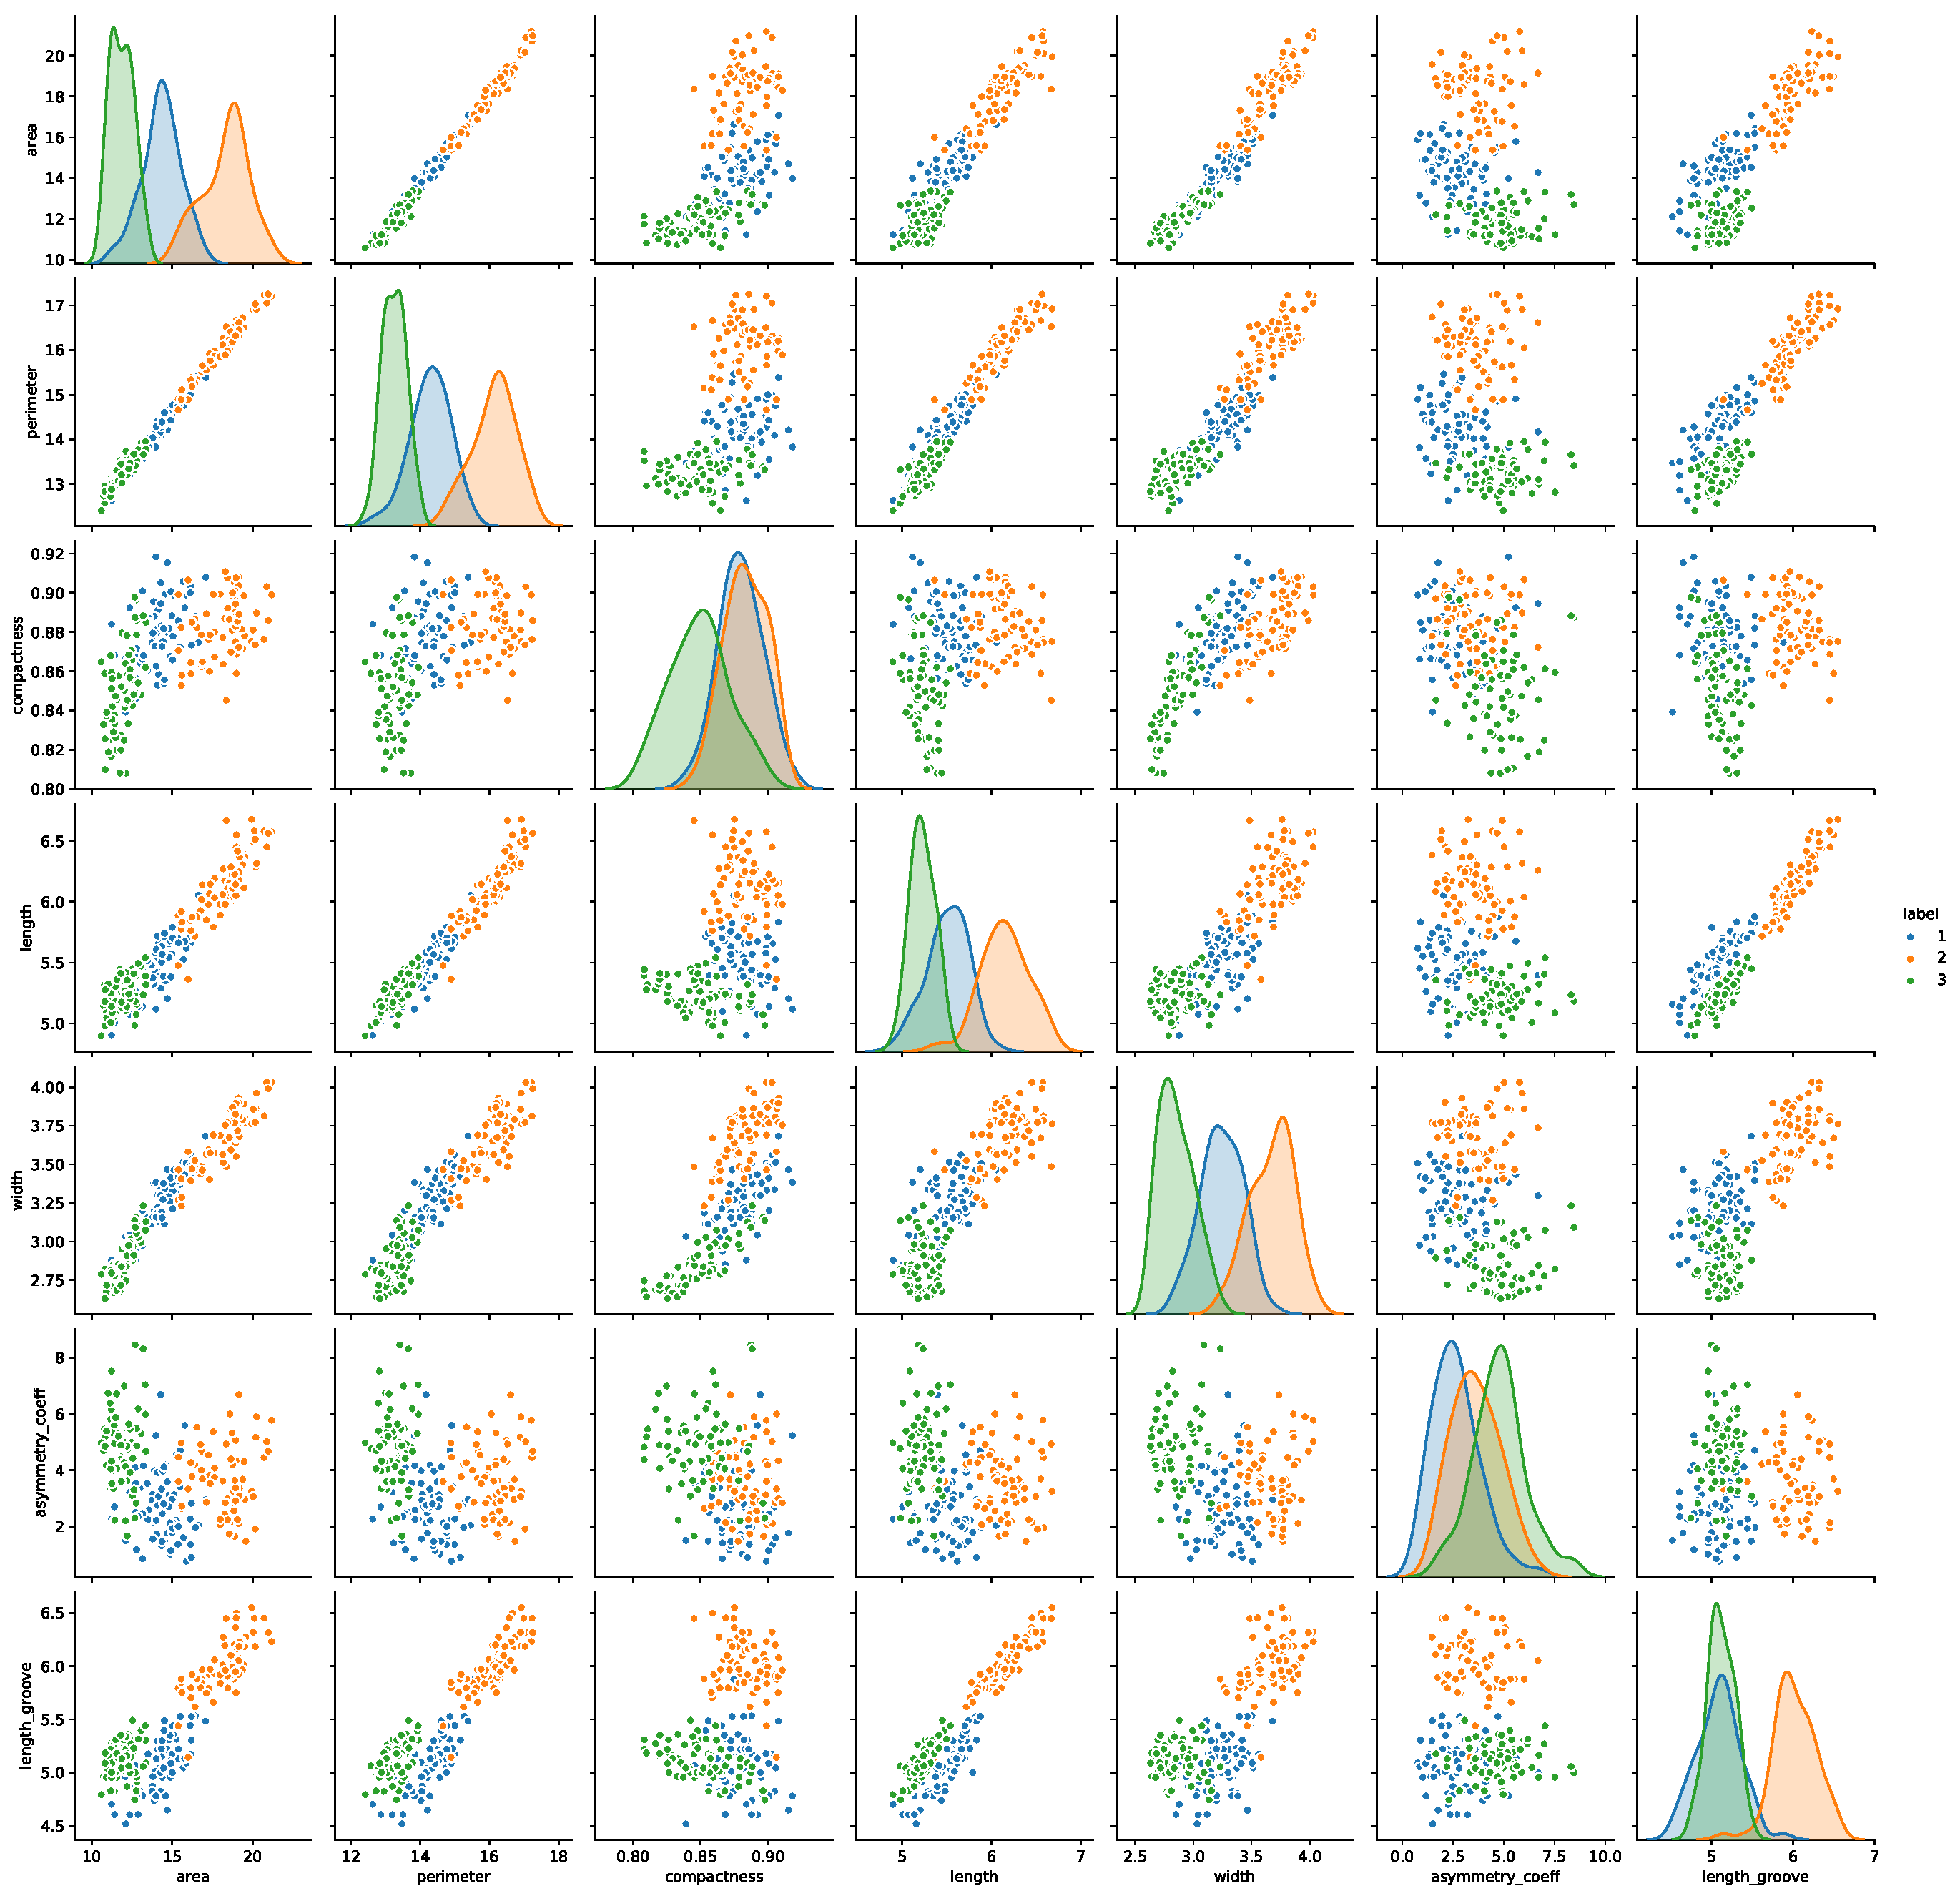
\includepdf[pages=-,scale=.4]{images/seeds_pairplot.pdf}
\centering
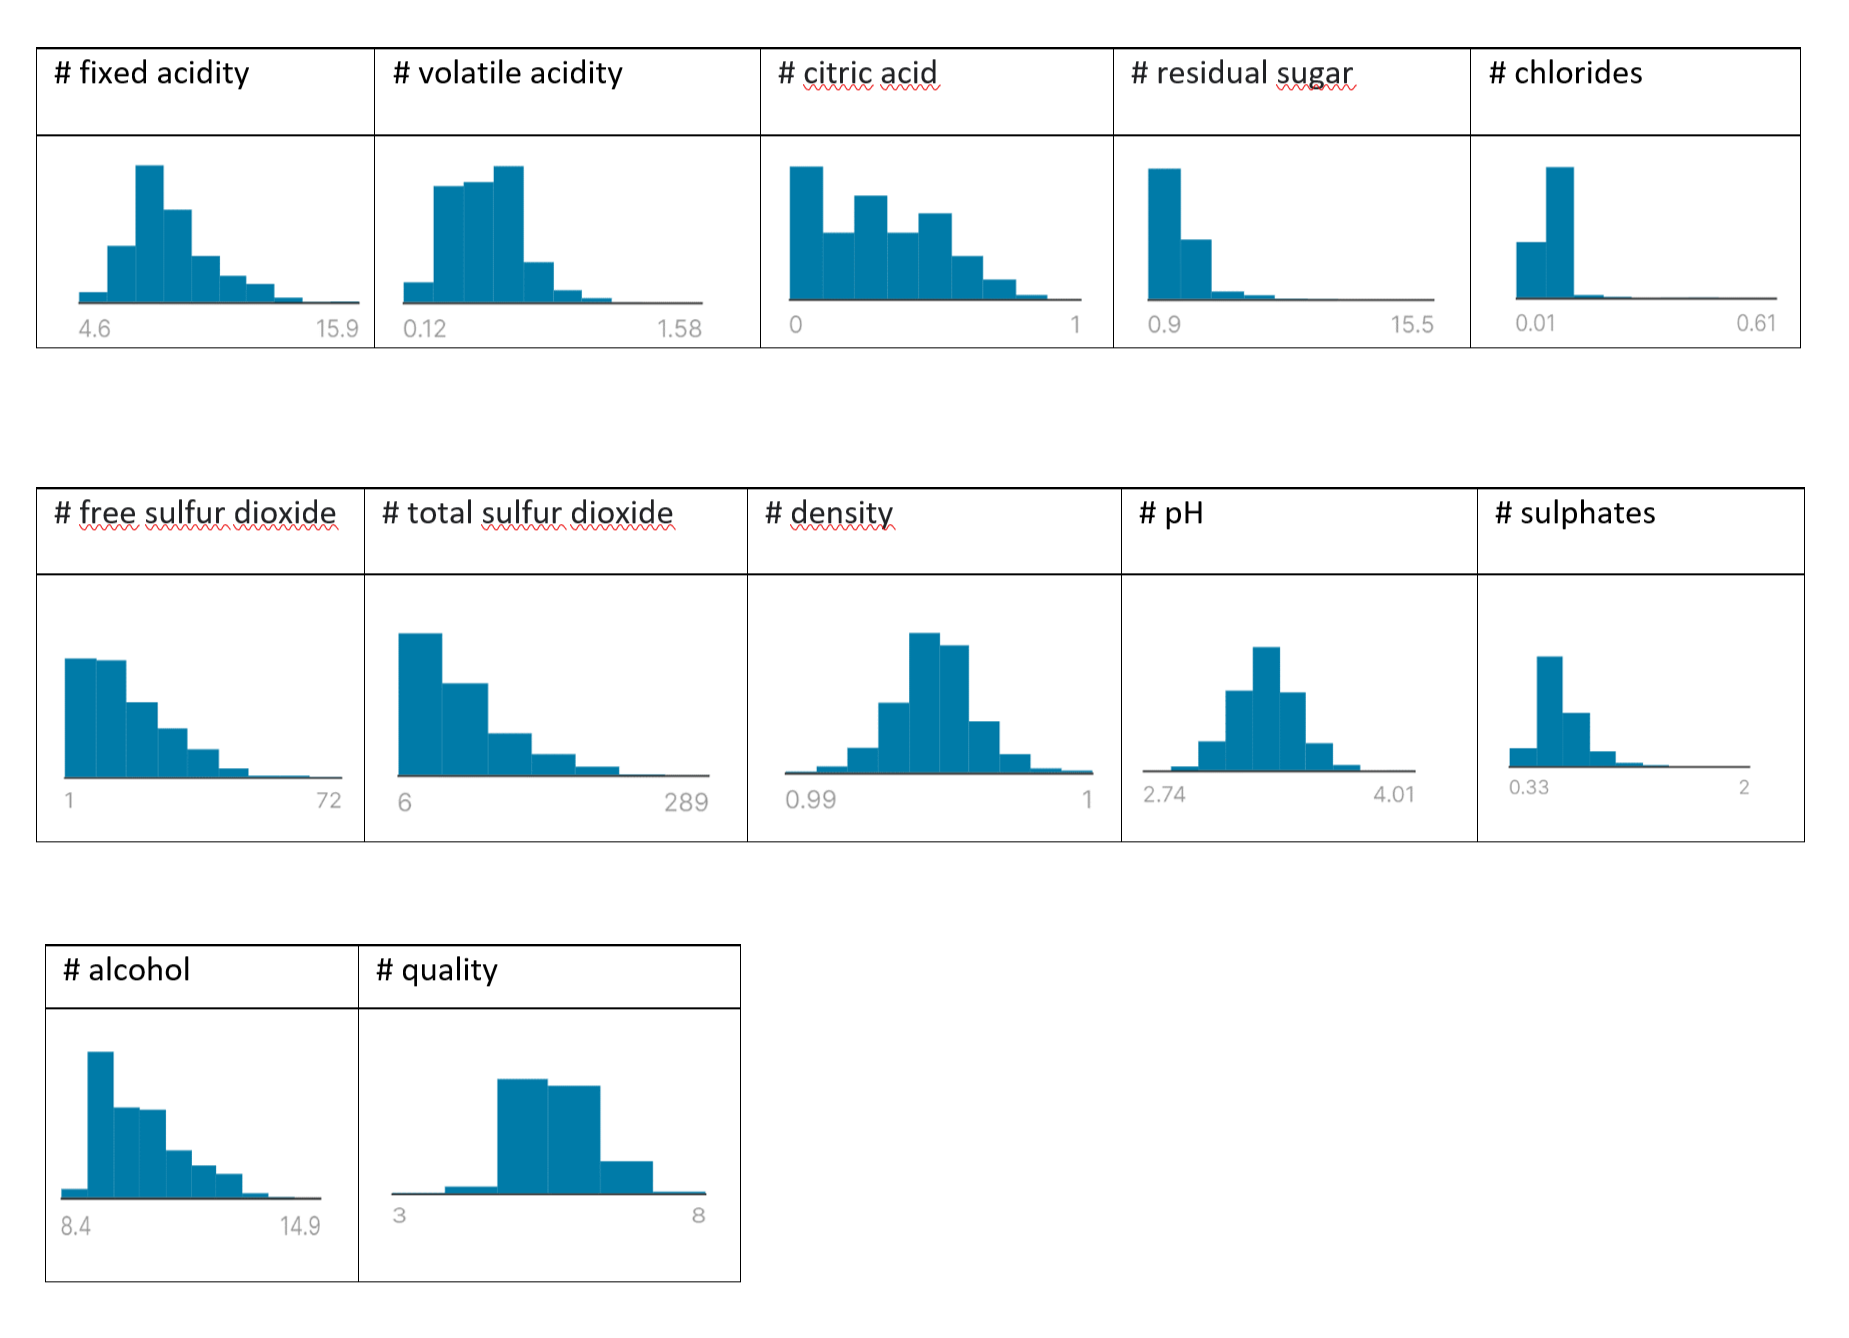
\includegraphics[width=1\textwidth]{images/wine_table1.PNG}
\caption{Spread of each attribute of the wine quality data set}
\label{fig:wine_stats}
\end{figure}